% Apresentação em Beamer (16:9), cerca de 10 a 15 minutos.
% Compilar: latexmk -pdf slides.tex   (ou "make slides" na raiz do repositório)
% Para ver as notas do apresentador numa segunda tela, troque "hide notes" por
% "show notes on second screen=right" na linha \setbeameroption abaixo.
\documentclass[aspectratio=169,11pt]{beamer}

\usepackage[T1]{fontenc}
\usepackage[utf8]{inputenc}
\usepackage[brazil]{babel}
\usepackage{lmodern}
\usepackage{graphicx}
\usepackage{booktabs}
\usepackage{pgfpages}
\setbeameroption{hide notes}

\graphicspath{{../graficos/}}

% Visual: fundo branco, um azul de destaque e o vermelho da BYD, como no site.
\definecolor{destaque}{HTML}{1747C8}
\definecolor{byd}{HTML}{C8102E}
\definecolor{tinta}{HTML}{16202B}
\definecolor{cinza}{HTML}{5A6878}
\usetheme{default}
\usefonttheme{structurebold}
\setbeamertemplate{navigation symbols}{}
\setbeamercolor{normal text}{fg=tinta}
\setbeamercolor{structure}{fg=destaque}
\setbeamercolor{frametitle}{fg=tinta}
\setbeamerfont{frametitle}{size=\Large,series=\bfseries}
\setbeamertemplate{frametitle}{\vspace{6pt}\insertframetitle\par\vspace{-2pt}}
\setbeamertemplate{footline}{\hfill{\color{cinza}\footnotesize\insertframenumber}\hspace{10pt}\vspace{6pt}}
\setbeamertemplate{itemize items}[circle]
\setbeamersize{text margin left=9mm,text margin right=9mm}

% Número grande com uma linha de explicação embaixo.
\newcommand{\numero}[2]{{\fontsize{24}{27}\selectfont\bfseries\color{destaque}#1}\par\vspace{3pt}{\small\color{cinza}#2}\par}
% Versão menor, para números compostos que não cabem na coluna em tamanho grande.
\newcommand{\numerom}[2]{{\fontsize{15}{18}\selectfont\bfseries\color{destaque}#1}\par\vspace{3pt}{\small\color{cinza}#2}\par}
\newcommand{\fontedados}[1]{\par\vspace{2pt}{\scriptsize\color{cinza}Fonte: #1}}

% PREENCHER: nomes dos integrantes, professor(a) e disciplina.
\title{Concentrado, mas contestado}
\subtitle{A rivalidade no mercado brasileiro de carros 100\% elétricos, 2020--2026}
\author{Nomes dos integrantes do grupo}
\institute{AP1 $\cdot$ Ibmec}
\date{Novembro de 2026}

\begin{document}

% 1
\begin{frame}[plain]
\vfill
{\color{cinza}\small AP1 $\cdot$ Rivalidade setorial $\cdot$ Ibmec}\par\vspace{8pt}
{\fontsize{32}{36}\selectfont\bfseries Concentrado, mas contestado}\par\vspace{8pt}
{\Large A rivalidade no mercado brasileiro de carros 100\% elétricos, 2020--2026}\par\vspace{22pt}
{\insertauthor}\par
{\color{cinza}\insertdate}
\vfill
\note{Abrir com a pergunta, não com o sumário. 20 segundos.}
\end{frame}

% 2
\begin{frame}{Uma marca vende 7 de cada 10 elétricos. Isso é pouca rivalidade?}
\begin{columns}[T]
\column{.54\textwidth}
\textbf{Pergunta}\par
Qual é a intensidade da rivalidade entre os concorrentes no mercado brasileiro de carros 100\% elétricos, e o que a explica?
\vspace{14pt}

\textbf{Resposta}\par
O mercado é altamente concentrado e, ao mesmo tempo, intensamente disputado. Quem ameaça a líder é outra marca com a mesma estratégia de custo, não o imposto de importação.
\column{.40\textwidth}
\numero{99$\times$}{crescimento do mercado, 2020 a 2025}
\vspace{10pt}
\numero{72\%}{participação da BYD em 2025}
\vspace{10pt}
\numero{$-$10,1 p.p.}{na BYD quando o Geely EX2 chegou}
\end{columns}
\note{Dizer a conclusão logo. O resto da apresentação é a evidência, em oito passos. Dados todos públicos: Fenabrave, ABVE, Comex Stat, FIPE, Banco Central.}
\end{frame}

% 3
\begin{frame}{1. O mercado explodiu: de 801 para 79 mil carros por ano}
\begin{columns}[c]
\column{.64\textwidth}
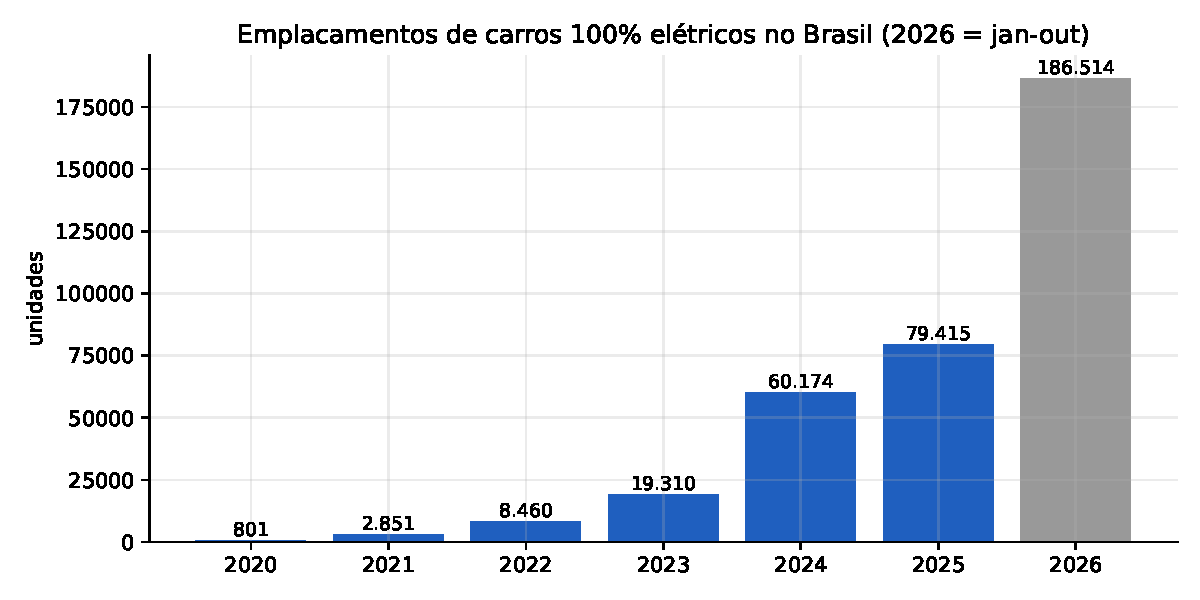
\includegraphics[width=\linewidth]{01_tamanho_mercado.pdf}
\column{.31\textwidth}
\numero{151\%}{de crescimento médio ao ano, 2020 a 2025}
\vspace{12pt}
\numero{186.514}{só de janeiro a outubro de 2026}
\end{columns}
\fontedados{ABVE (2020 a 2023) e Fenabrave (2024 em diante).}
\note{Por que importa para a rivalidade: em mercado que dobra todo ano, cada marca cresce sem tirar cliente da outra (Porter). Guardar essa ideia para o fim.}
\end{frame}

% 4
\begin{frame}{2. De um nicho premium disputado a uma marca dominante}
\begin{columns}[c]
\column{.64\textwidth}
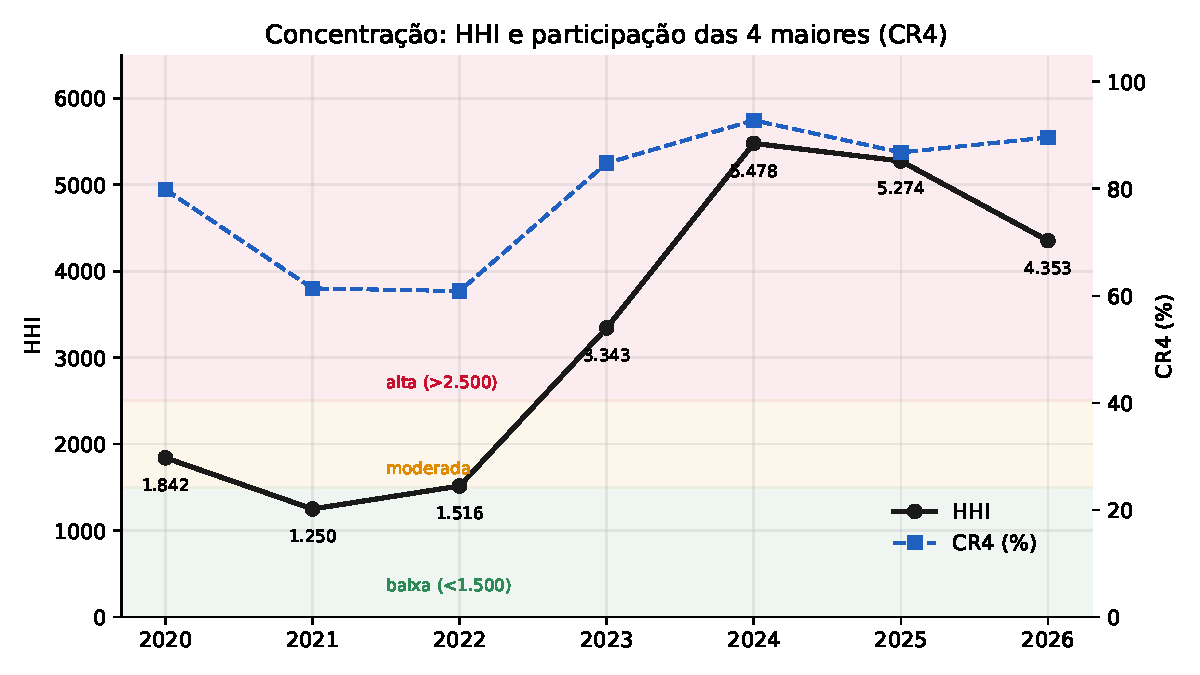
\includegraphics[width=\linewidth]{03_hhi_cr4.pdf}
\column{.31\textwidth}
\numerom{1.516 $\rightarrow$ 5.478}{HHI de 2022 para 2024}
\vspace{12pt}
\numerom{51\% $\rightarrow$ 2\%}{Volvo, BMW, Mercedes e Porsche somadas, 2022 para 2026}
\end{columns}
\fontedados{ABVE e Fenabrave. HHI: soma dos quadrados das participações; acima de 2.500, concentração alta.}
\note{Explicar o HHI em uma frase. A BYD entra em 2023 com o Dolphin abaixo de R\$ 150 mil. O índice passa o de telefonia móvel e aviação doméstica.}
\end{frame}

% 5
\begin{frame}{3. A virada não é efeito das nossas estimativas}
\begin{columns}[c]
\column{.64\textwidth}
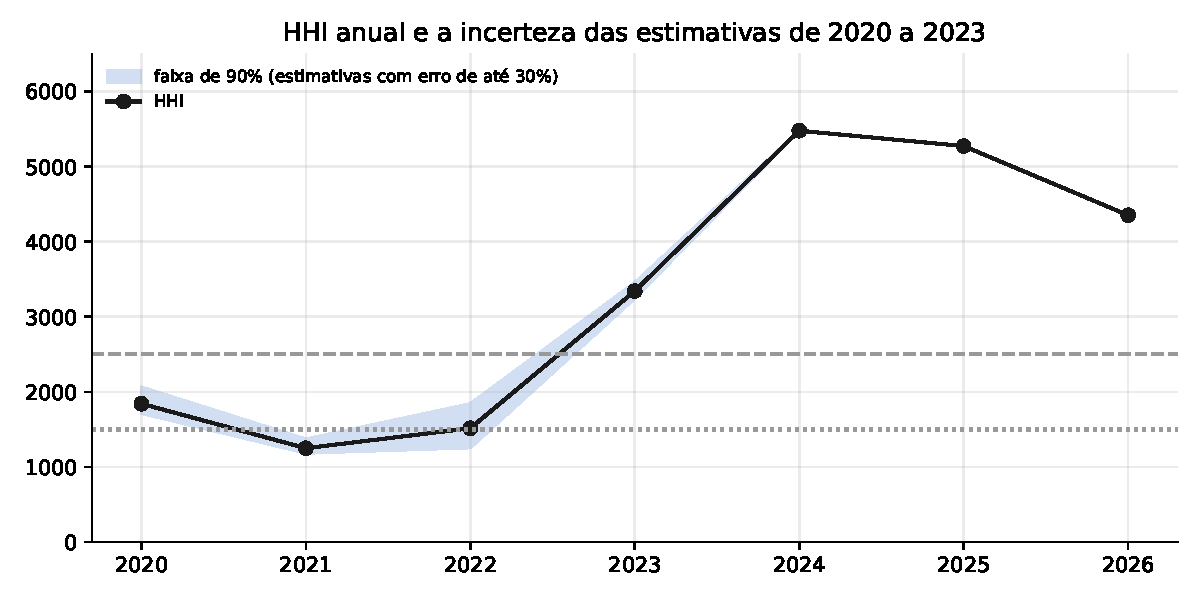
\includegraphics[width=\linewidth]{11_montecarlo_hhi.pdf}
\column{.31\textwidth}
Antes de 2024 não há ranking oficial por marca: a divisão é estimativa do grupo.
\vspace{10pt}

Refizemos a conta 5.000 vezes, errando cada estimativa em até 30\%.
\vspace{10pt}

\numerom{3.244 a 3.457}{HHI de 2023 em qualquer cenário: sempre alta}
\end{columns}
\note{Ser franco sobre a limitação e mostrar que foi testada. Em 2022 não dá para dizer se era baixa ou moderada (47\% contra 53\% das simulações). Em 2023 não há dúvida.}
\end{frame}

% 6
\begin{frame}{4. ``Quase monopólio'' só vale se o mercado for só o de elétricos}
\begin{columns}[c]
\column{.60\textwidth}
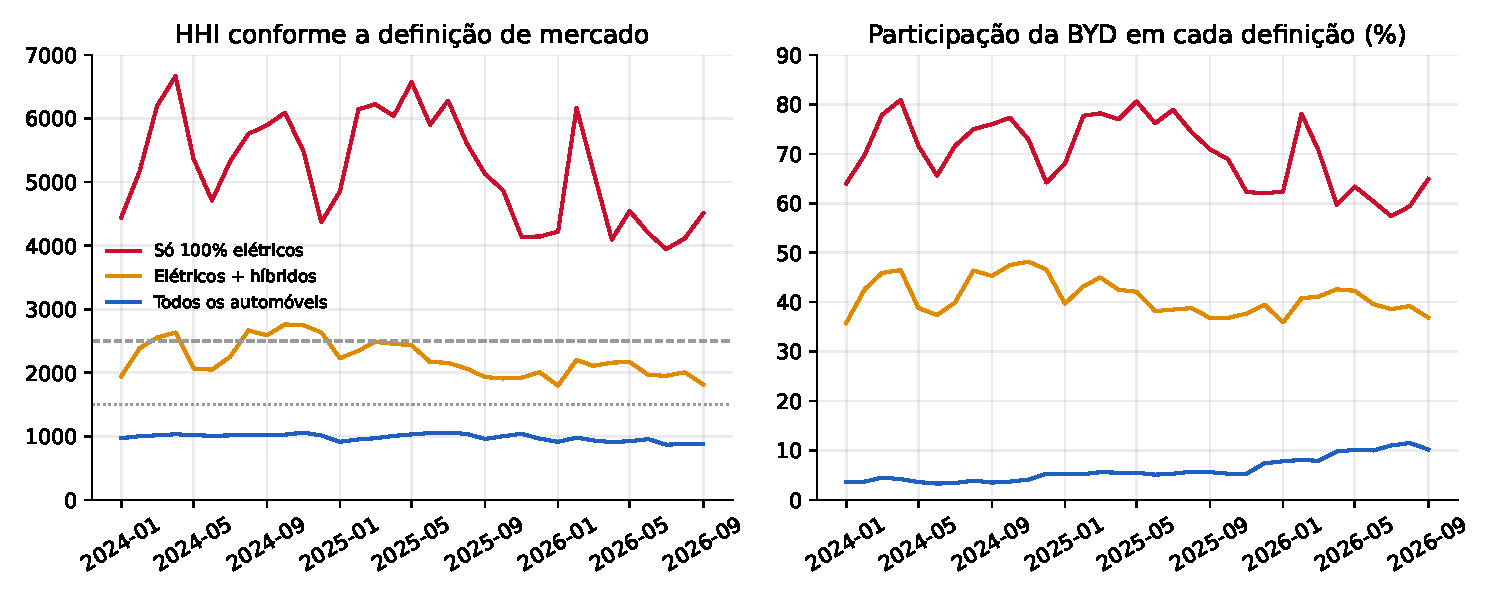
\includegraphics[width=\linewidth]{10_definicoes_mercado.pdf}
\column{.36\textwidth}
\small
\begin{tabular}{@{}lrr@{}}
\toprule
Mercado & HHI & BYD \\
\midrule
Só elétricos & 4.553 & 64,1\% \\
Com híbridos & 2.020 & 39,7\% \\
Todos os carros & 916 & 9,6\% \\
\bottomrule
\end{tabular}
\vspace{10pt}

Média de 2026. No mercado de automóveis como um todo, a BYD ainda é desafiante.
\end{columns}
\fontedados{Fenabrave, janeiro de 2024 a setembro de 2026.}
\note{Quem compra um Dolphin também olhou híbrido e combustão. O trabalho mede a rivalidade dentro do segmento elétrico, e é bom deixar isso claro.}
\end{frame}

% 7
\begin{frame}{5. Quem abalou a BYD foi um rival, não o imposto}
\begin{columns}[c]
\column{.60\textwidth}
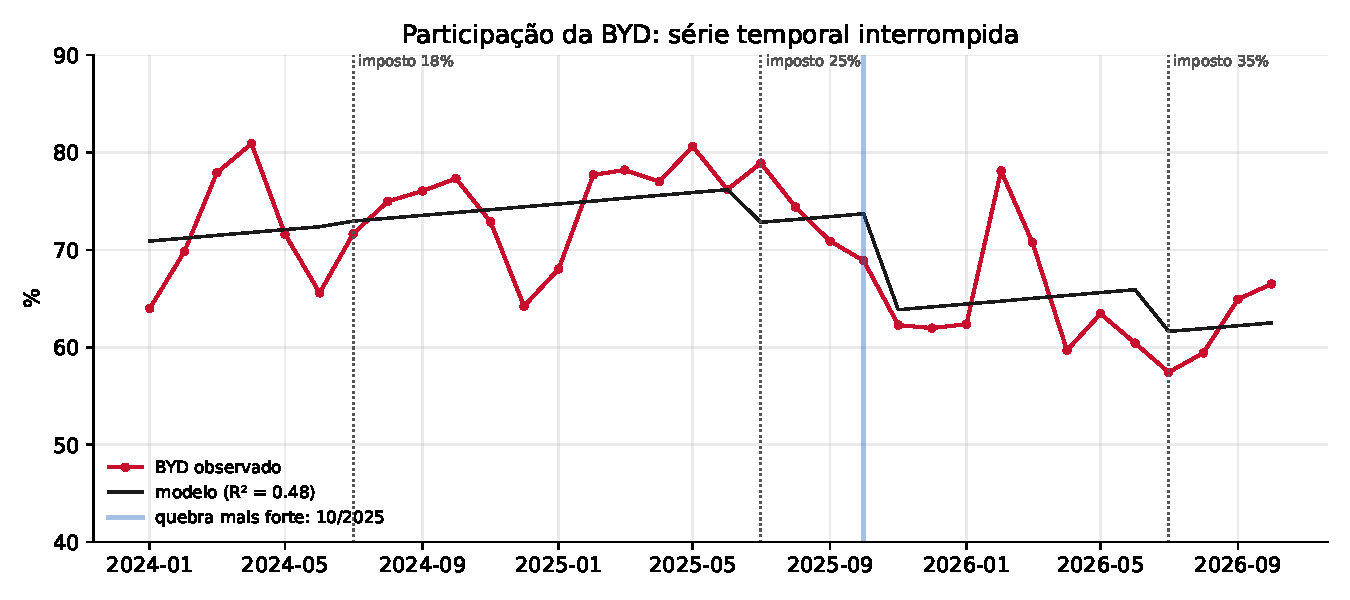
\includegraphics[width=\linewidth]{12_serie_interrompida_byd.pdf}
\column{.36\textwidth}
\small
\begin{tabular}{@{}lrr@{}}
\toprule
Evento & Efeito & $p$ \\
\midrule
Imposto 18\% & $+$0,3 & 0,933 \\
Imposto 25\% & $-$3,6 & 0,255 \\
\textbf{Geely EX2} & \textbf{$-$10,1} & \textbf{0,001} \\
Imposto 35\% & $-$4,6 & 0,112 \\
\bottomrule
\end{tabular}
\vspace{8pt}

Efeito em pontos percentuais na participação da BYD. Um teste que procura a quebra sozinho aponta outubro de 2025, mês de lançamento do EX2.
\end{columns}
\note{Este é o slide central. Método: série temporal interrompida, 34 meses. Só um evento tem efeito claro. Ressalva: poucos meses, o sinal é mais confiável que o tamanho.}
\end{frame}

% 8
\begin{frame}{6. O imposto mudou a data das importações, não as participações}
\begin{columns}[c]
\column{.64\textwidth}
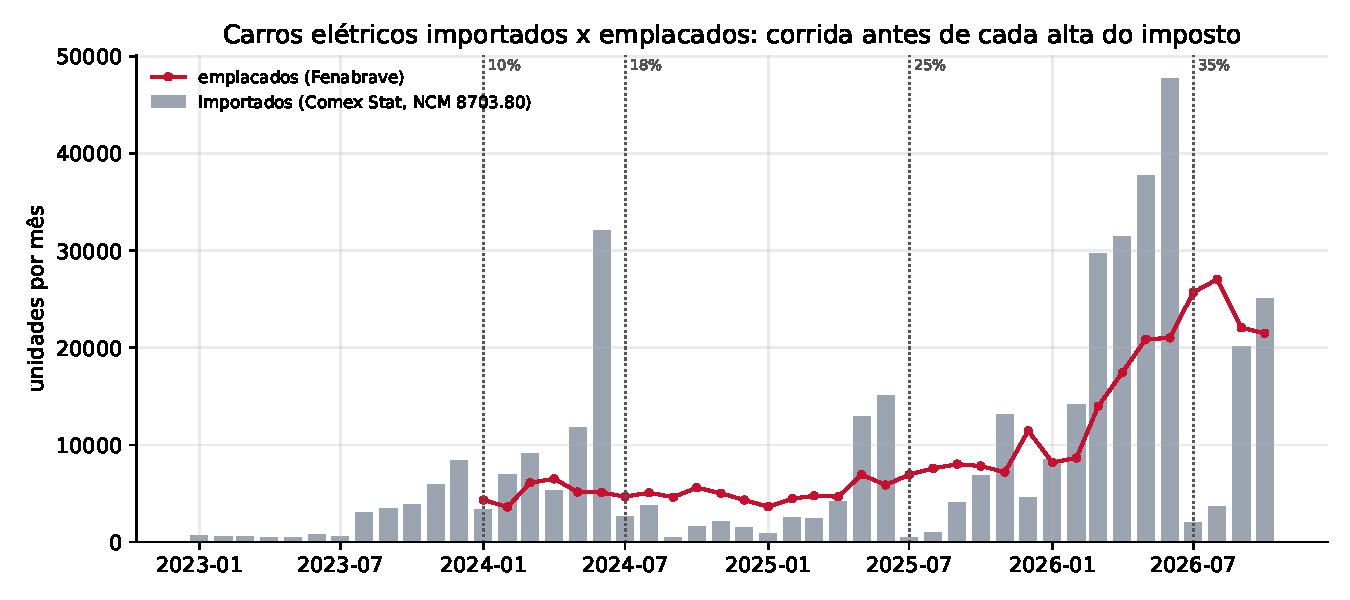
\includegraphics[width=\linewidth]{13_importacoes_estoque.pdf}
\column{.31\textwidth}
\numerom{7,2$\times$ \ 5,8$\times$ \ 4,5$\times$}{importações nos 3 meses antes de cada alta, em relação aos 3 meses depois}
\vspace{10pt}

Comparando quem só importa com quem monta aqui: sinal esperado, mas não significativo ($p = 0{,}45$).
\end{columns}
\fontedados{Comex Stat (NCM 8703.80.00) e Fenabrave.}
\note{As marcas anteciparam embarques e venderam o estoque com a alíquota antiga. Por isso o imposto ainda não aparece nas participações. 97\% das unidades vêm da China.}
\end{frame}

% 9
\begin{frame}{7. A rivalidade aparece no preço e na variedade}
\begin{columns}[c]
\column{.62\textwidth}
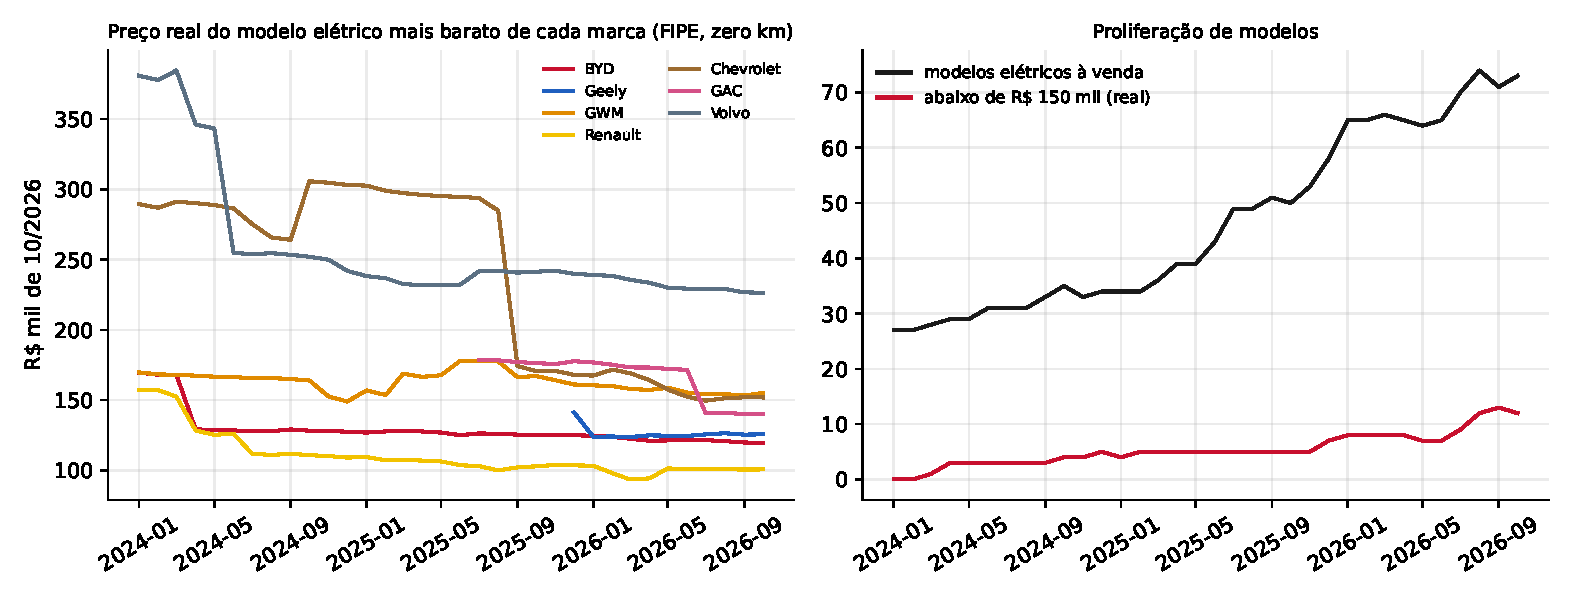
\includegraphics[width=\linewidth]{15_precos_fipe.pdf}
\column{.34\textwidth}
\numerom{R\$ 157 mil $\rightarrow$ R\$ 101 mil}{elétrico mais barato, em valores reais}
\vspace{8pt}
\numero{27 $\rightarrow$ 73}{versões à venda}
\vspace{8pt}
\numero{$-$26\%}{preço de uma marca chinesa com a mesma potência e bateria}
\end{columns}
\fontedados{Tabela FIPE, janeiro de 2024 a outubro de 2026, corrigida pelo IPCA; regressão hedônica com 68 modelos.}
\note{Se a participação da líder quase não cede, a disputa está no que o consumidor paga e pode escolher. É a liderança em custo de Porter, medida.}
\end{frame}

% 10
\begin{frame}{8. Para onde vai: sabemos o mecanismo, não o teto}
\begin{columns}[c]
\column{.64\textwidth}
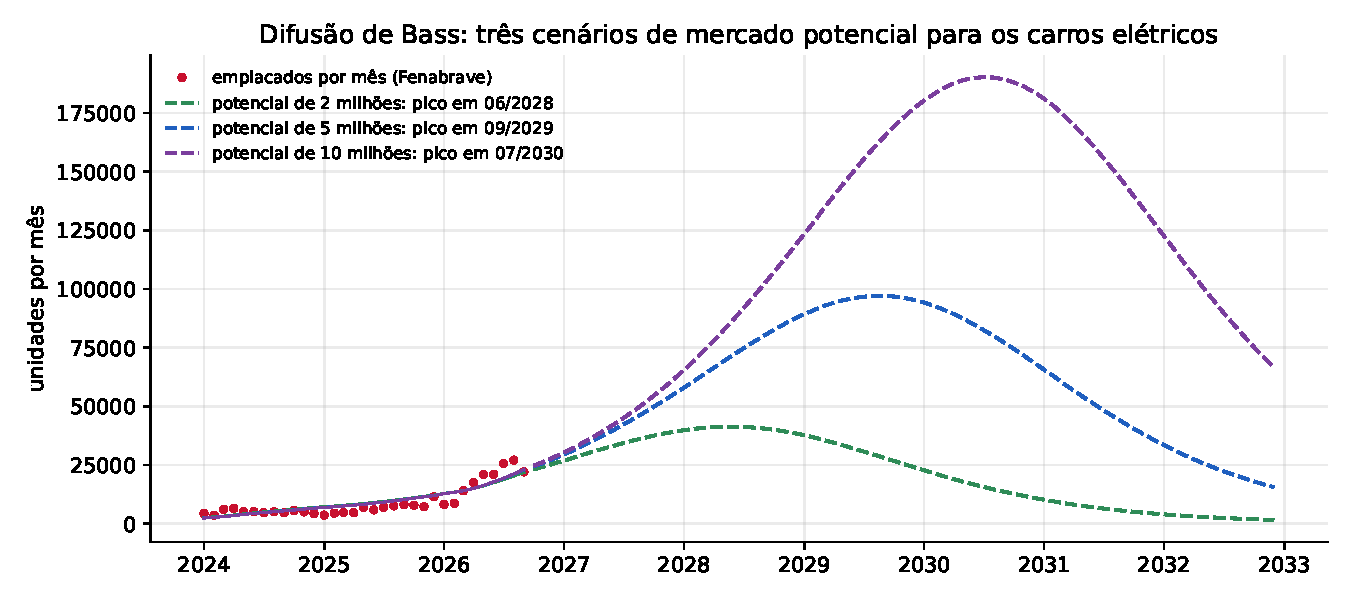
\includegraphics[width=\linewidth]{14_bass_difusao.pdf}
\column{.31\textwidth}
\numerom{13 meses}{para as vendas mensais dobrarem}
\vspace{10pt}

Mercado final de 2, 5 ou 10 milhões se ajusta igualmente bem aos dados. O pico viria entre 2028 e 2030.
\vspace{8pt}

São cenários, não previsões.
\end{columns}
\fontedados{Fenabrave; curva de difusão de Bass.}
\note{A adoção se espalha por imitação. Não fazemos previsão: o modelo de aprendizado de máquina empata com ``repetir o mês passado'' (R2 de 0,82 contra 0,80).}
\end{frame}

% 11
\begin{frame}{O que isso significa: rivalidade em alta, apesar da concentração}
\begin{columns}[T]
\column{.47\textwidth}
\textbf{As cinco forças, 2022 e 2026}\par\vspace{4pt}
\small
\begin{tabular}{@{}lcc@{}}
\toprule
Força (1 fraca, 5 forte) & 2022 & 2026 \\
\midrule
Rivalidade & 3 & \textbf{4} \\
Novos entrantes & 4 & 3 \\
Fornecedores & 4 & 3 \\
Compradores & 2 & \textbf{4} \\
Substitutos & 4 & 4 \\
\bottomrule
\end{tabular}\par\vspace{4pt}
{\scriptsize\color{cinza}Avaliação qualitativa do grupo.}
\column{.49\textwidth}
\begin{itemize}
\item \textbf{Custo venceu diferenciação.} As chinesas lideram por custo; as premium ficaram em um nicho de 2\%.
\item \textbf{A briga agora é entre iguais.} Mesma estratégia genérica, competição por preço.
\item \textbf{Produzir no Brasil virou condição.} Com 35\% de imposto, a barreira para quem só importa subiu.
\end{itemize}
\end{columns}
\note{Ligar com a teoria: Porter (forças e estratégias genéricas), Uppsala (importar, montar, produzir), Chandler (estrutura segue estratégia). As notas das forças são julgamento do grupo, não medida.}
\end{frame}

% 12
\begin{frame}{O que este trabalho não mostra}
\begin{itemize}
\item A divisão por marca de 2020 a 2023 é \textbf{estimativa do grupo}. A conclusão central não depende dela, mas os números desses anos são aproximados.
\item A Fenabrave publica só as 15 maiores marcas por mês; outubro de 2026 é parcial.
\item São 33 meses de dados mensais completos: bastam para ver a direção dos efeitos, não para medir o tamanho com precisão.
\item Potência, bateria e datas de montagem local foram compiladas pelo grupo e precisam de conferência.
\end{itemize}
\note{Dizer isso antes que perguntem aumenta a confiança no resto.}
\end{frame}

% 13
\begin{frame}{Próximo passo: ouvir o consumidor}
\begin{columns}[T]
\column{.52\textwidth}
Falta o lado da demanda. Preparamos um questionário baseado no modelo de aceitação de tecnologia (TAM, Davis, 1989):
\begin{itemize}
\item 10 afirmações, escala de 1 a 5;
\item utilidade percebida, facilidade de uso, atitude e intenção de compra;
\item a aplicar na turma.
\end{itemize}
\column{.42\textwidth}
\textbf{Exemplos de itens}\par\vspace{4pt}
{\small ``Um carro elétrico me faria economizar com combustível e manutenção.''\par\vspace{6pt}
``Seria fácil encontrar onde recarregar um carro elétrico.''\par\vspace{6pt}
``Pretendo comprar um carro elétrico no meu próximo carro.''}
\end{columns}
\vspace{10pt}
{\small\color{cinza}Ainda não há respostas reais; por isso não apresentamos resultados desta etapa.}
\note{Se houver tempo, convidar a turma a responder. Não mostrar os gráficos de exemplo com dados simulados.}
\end{frame}

% 14
\begin{frame}{Concentrado, mas contestado}
\begin{columns}[c]
\column{.60\textwidth}
\begin{itemize}
\item O mercado cresceu 99 vezes e ficou nas mãos de uma marca.
\item A líder só perdeu espaço quando chegou um rival com a mesma estratégia de custo.
\item O imposto mudou quando os carros chegam, não quem os vende.
\item A disputa aparece no preço e na variedade: entrada um terço mais barata e quase três vezes mais modelos.
\end{itemize}
\column{.34\textwidth}
\textbf{Site interativo, artigo e dados}\par\vspace{6pt}
{\small\texttt{marceufilho.github.io/\\carros-eletricos}}
\end{columns}
\note{Fechar repetindo a frase do título. Deixar este slide na tela durante as perguntas.}
\end{frame}

% ---------------- slides de apoio (para perguntas) ----------------
\appendix

\begin{frame}{Apoio: série temporal interrompida, tabela completa}
\small
\centering
\begin{tabular}{lrrr}
\toprule
Termo & Coeficiente (p.p.) & Erro-padrão & $p$-valor \\
\midrule
Constante & 70,90 & 2,54 & 0,000 \\
Tendência (por mês) & 0,29 & 0,23 & 0,211 \\
Imposto de 18\% (jul/2024) & 0,29 & 3,40 & 0,933 \\
Imposto de 25\% e Camaçari (jul/2025) & $-$3,65 & 3,20 & 0,255 \\
Geely EX2 em volume (nov/2025) & $-$10,15 & 3,12 & 0,001 \\
Imposto de 35\% (jul/2026) & $-$4,57 & 2,88 & 0,112 \\
\bottomrule
\end{tabular}
\par\vspace{8pt}
{\footnotesize\color{cinza}Participação mensal da BYD, 34 meses (jan/2024 a out/2026), erros-padrão HAC com 2 defasagens, $R^2 = 0{,}48$.\\
Quebra estrutural em data desconhecida: outubro de 2025 ($F = 10{,}8$).}
\end{frame}

\begin{frame}{Apoio: regressão hedônica e painel do imposto}
\begin{columns}[T]
\column{.52\textwidth}
\small
\textbf{Logaritmo do preço (68 modelos, $R^2 = 0{,}87$)}\par\vspace{4pt}
\begin{tabular}{@{}lrr@{}}
\toprule
Termo & Coef. & $p$ \\
\midrule
Log da bateria (kWh) & 0,785 & 0,000 \\
Log da potência (cv) & 0,365 & 0,009 \\
Marca chinesa & $-$0,302 & 0,000 \\
Marca premium & 0,218 & 0,002 \\
\bottomrule
\end{tabular}
\column{.44\textwidth}
\small
\textbf{Painel marca $\times$ mês}\par\vspace{4pt}
13 marcas, 429 observações, efeitos fixos de marca e de mês, erros agrupados por marca.\par\vspace{6pt}
Exposição ao imposto: coeficiente de $-$0,039, erro-padrão de 0,052, $p = 0{,}453$.\par\vspace{6pt}
Não se distingue de zero.
\end{columns}
\end{frame}

\begin{frame}{Apoio: três grupos estratégicos (k-means)}
\begin{columns}[c]
\column{.52\textwidth}
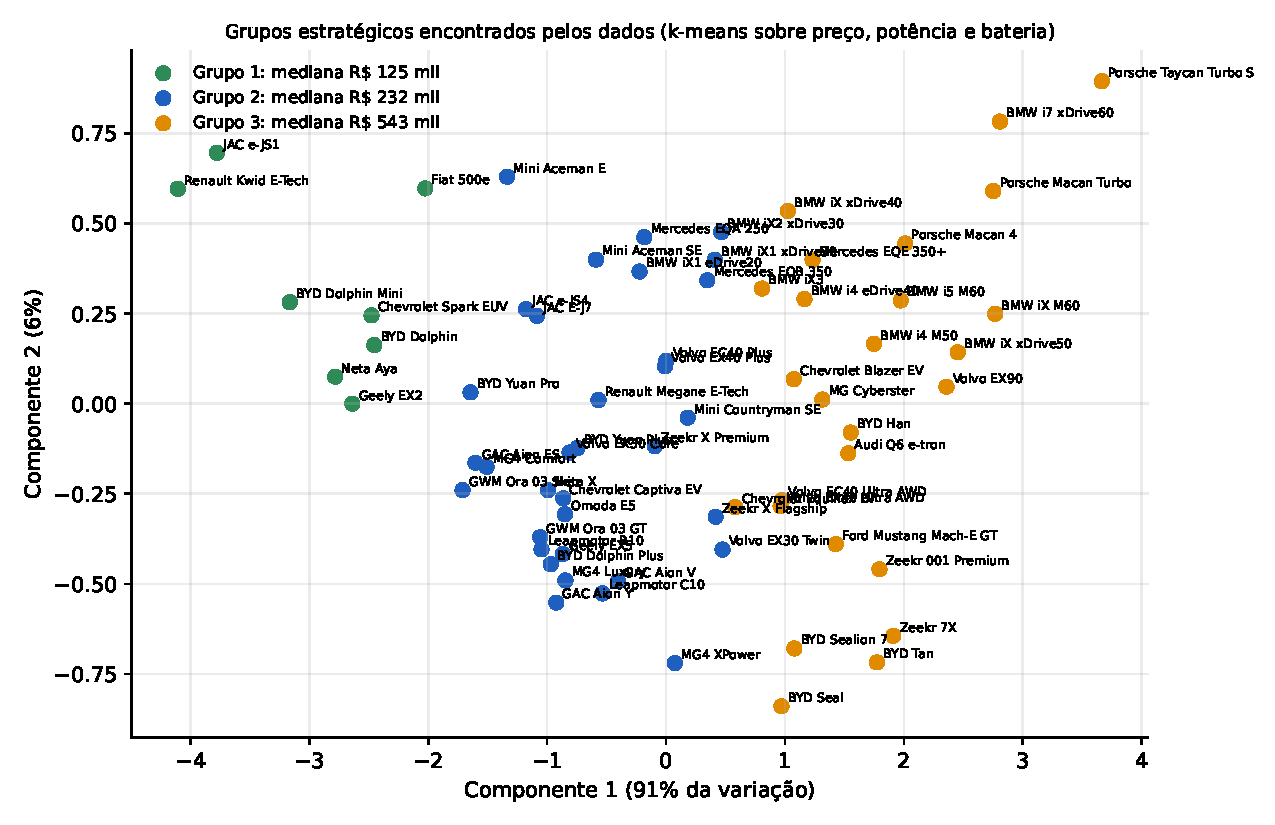
\includegraphics[width=\linewidth]{17_grupos_estrategicos.pdf}
\column{.44\textwidth}
\small
\begin{tabular}{@{}lrrr@{}}
\toprule
Grupo & Modelos & Preço mediano & Chinesas \\
\midrule
Entrada & 8 & R\$ 125 mil & 62\% \\
Intermediário & 34 & R\$ 232 mil & 59\% \\
Topo & 26 & R\$ 543 mil & 27\% \\
\bottomrule
\end{tabular}
\par\vspace{8pt}
Agrupamento por preço, potência e bateria; silhueta de 0,47.
\end{columns}
\end{frame}

\begin{frame}{Apoio: fontes de dados e referências}
\footnotesize
\textbf{Dados.} Fenabrave, informativos mensais (jan/2024 a out/2026); ABVE, série histórica de eletrificados; MDIC, Comex Stat, NCM 8703.80.00; Tabela FIPE; Banco Central do Brasil, SGS.
\vspace{8pt}

\textbf{Referências.}\par
BASS, F. M. A new product growth for model consumer durables. \textit{Management Science}, 1969.\par
CHANDLER, A. D. \textit{Strategy and structure}. Cambridge: MIT Press, 1962.\par
DAVIS, F. D. Perceived usefulness, perceived ease of use, and user acceptance of information technology. \textit{MIS Quarterly}, 1989.\par
HYMER, S.; PASHIGIAN, P. Turnover of firms as a measure of market behavior. \textit{The Review of Economics and Statistics}, 1962.\par
JOHANSON, J.; VAHLNE, J.-E. The internationalization process of the firm. \textit{Journal of International Business Studies}, 1977.\par
MINTZBERG, H. The strategy concept I: five Ps for strategy. \textit{California Management Review}, 1987.\par
PORTER, M. E. How competitive forces shape strategy. \textit{Harvard Business Review}, 1979.\par
PORTER, M. E. \textit{Competitive strategy}. New York: Free Press, 1980.
\end{frame}

\end{document}
